\documentclass[12pt,a4paper]{article}
\usepackage[utf8]{inputenc}
\usepackage[spanish]{babel}
\usepackage{graphicx}
\usepackage{geometry}
\usepackage{hyperref}
\usepackage{listings}
\usepackage{xcolor}
\usepackage{float}
\usepackage{array}
\usepackage{booktabs}
\usepackage{fancyhdr}
\usepackage{setspace}

\geometry{left=2.5cm, right=2.5cm, top=2.5cm, bottom=2.5cm}
\setlength{\headheight}{14.5pt}
\setstretch{1.5}

\lstset{
    language=Python,
    basicstyle=\footnotesize\ttfamily,
    keywordstyle=\color{blue},
    commentstyle=\color{gray},
    stringstyle=\color{red},
    numbers=left,
    numberstyle=\tiny,
    frame=single,
    breaklines=true,
    tabsize=4
}

\pagestyle{fancy}
\fancyhf{}
\fancyhead[L]{PC4 - Programaci\'on Orientada a Objetos}
\fancyhead[R]{\thepage}
\renewcommand{\headrulewidth}{0.4pt}

\begin{document}

\onecolumn
\begin{titlepage}
    \centering
    \vspace*{2cm}
    {\Huge \textbf{Prototipo Zoom}}\\[0.5cm]
    {\Large Sistema de Videoconferencia por Sockets}\\[1.5cm]
    {\large \textbf{PC4 - Programaci\'on Orientada a Objetos}}\\[0.5cm]
    {\large Universidad}\\[0.3cm]
    {\large Facultad de Ingenier\'ia}\\[2cm]

    \begin{tabular}{ll}
        \textbf{Integrantes:} & \\
        & \\
        & \\
        & \\
    \end{tabular}\\[2cm]

    \textbf{Docente:}\\[1.8cm]

    \today
\end{titlepage}

\tableofcontents
\newpage

\section{Introducci\'on}

El presente documento describe el dise\~no e implementaci\'on de un \textbf{prototipo acad\'emico de videoconferencia} inspirado en Zoom, desarrollado en Python como parte del curso de Programaci\'on Orientada a Objetos (PC4).

El sistema emplea una arquitectura \textbf{cliente-servidor} basada en \textbf{sockets TCP} con un protocolo de mensajes en formato \textbf{JSON}. Cuenta con autenticaci\'on de usuarios, creaci\'on y gesti\'on de salas virtuales, chat en tiempo real, transferencia de archivos y transmisi\'on de video desde la c\'amara web.

\section{Objetivos}

\begin{itemize}
    \item Aplicar los principios de la POO: herencia, encapsulamiento, polimorfismo.
    \item Implementar una arquitectura cliente-servidor mediante sockets TCP.
    \item Desarrollar un protocolo de comunicaci\'on propio basado en JSON.
    \item Integrar m\'ultiples funcionalidades: login, salas, chat, archivos y video.
    \item Utilizar SQLite para la persistencia de informaci\'on.
    \item Emplear concurrencia con \texttt{threading} para atender m\'ultiples clientes.
\end{itemize}

\section{Tecnolog\'ias Utilizadas}

\begin{itemize}
    \item \textbf{Lenguaje:} Python 3.10+
    \item \textbf{Interfaz gr\'afica:} Tkinter
    \item \textbf{Comunicaci\'on:} Sockets TCP
    \item \textbf{Protocolo:} JSON sobre TCP
    \item \textbf{Base de datos:} SQLite
    \item \textbf{Concurrencia:} \texttt{threading}
    \item \textbf{Video:} OpenCV o ffmpeg
    \item \textbf{Im\'agenes:} Pillow
\end{itemize}

\section{Arquitectura del Sistema}

El sistema sigue un modelo cliente-servidor. El servidor centraliza las conexiones y act\'ua como intermediario. Cada cliente se conecta mediante TCP y el servidor asigna un hilo independiente por conexi\'on.

\IfFileExists{imagenes/arquitectura.png}{%
\begin{figure}[htbp]
    \centering
    \includegraphics[width=0.9\textwidth]{imagenes/arquitectura.png}
    \caption{Diagrama de arquitectura del sistema}
\end{figure}
}{}

\section{Base de Datos}

La base de datos SQLite contiene las siguientes tablas:

\begin{table}[htbp]
    \centering
    \begin{tabular}{p{3.5cm}p{10cm}}
    \toprule
    \textbf{Tabla} & \textbf{Columnas} \\
    \midrule
    Usuarios          & IdUsuario, Nombres, Correo, PasswordHash, Rol, Activo \\
    Salas             & IdSala, CodigoSala, Nombre, IdHost, Estado, FechaCreacion \\
    ParticipantesSala & IdParticipante, IdSala, IdUsuario, Estado, FechaIngreso \\
    SolicitudesSala   & IdSolicitud, IdSala, IdUsuario, Estado, FechaSolicitud \\
    Mensajes          & IdMensaje, IdSala, IdUsuario, Contenido, FechaEnvio \\
    ArchivosCompartidos & IdArchivo, IdSala, IdUsuario, NombreArchivo, RutaArchivo, Tamano, FechaSubida \\
    \bottomrule
    \end{tabular}
    \caption{Tablas de la base de datos}
\end{table}

\section{Diagrama de Casos de Uso}

\IfFileExists{imagenes/casos_de_uso.png}{%
\begin{figure}[htbp]
    \centering
    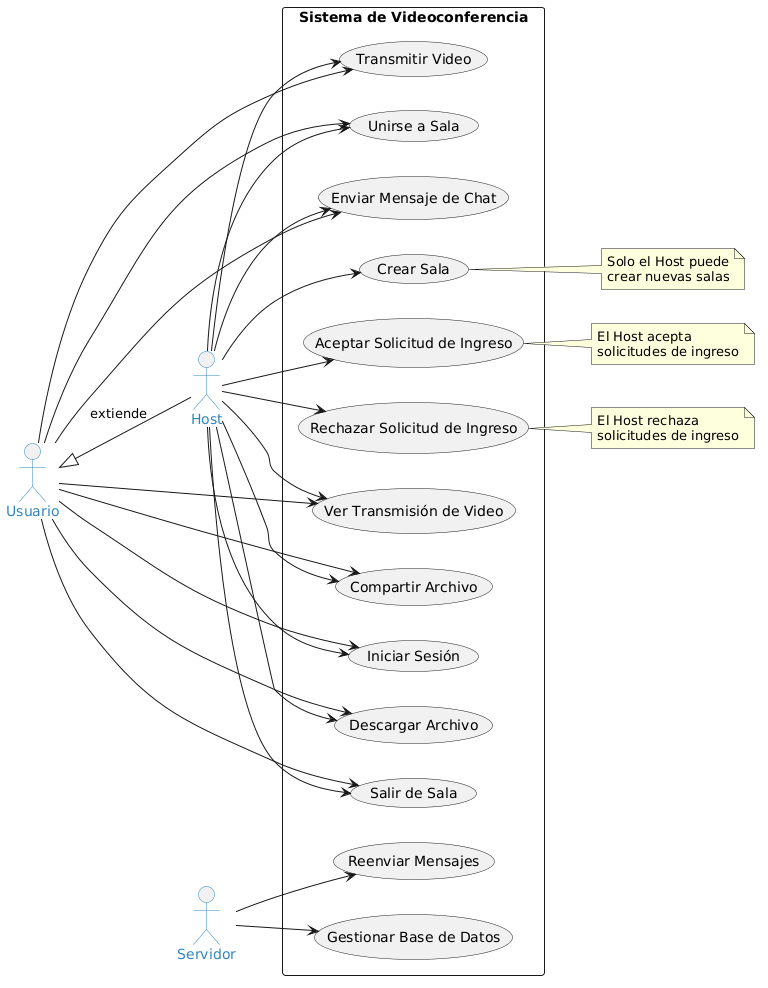
\includegraphics[width=0.9\textwidth]{imagenes/casos_de_uso.png}
    \caption{Diagrama de casos de uso del sistema}
\end{figure}
}{}

\section{Diagrama de Secuencia}

\IfFileExists{imagenes/secuencia.png}{%
\begin{figure}[htbp]
    \centering
    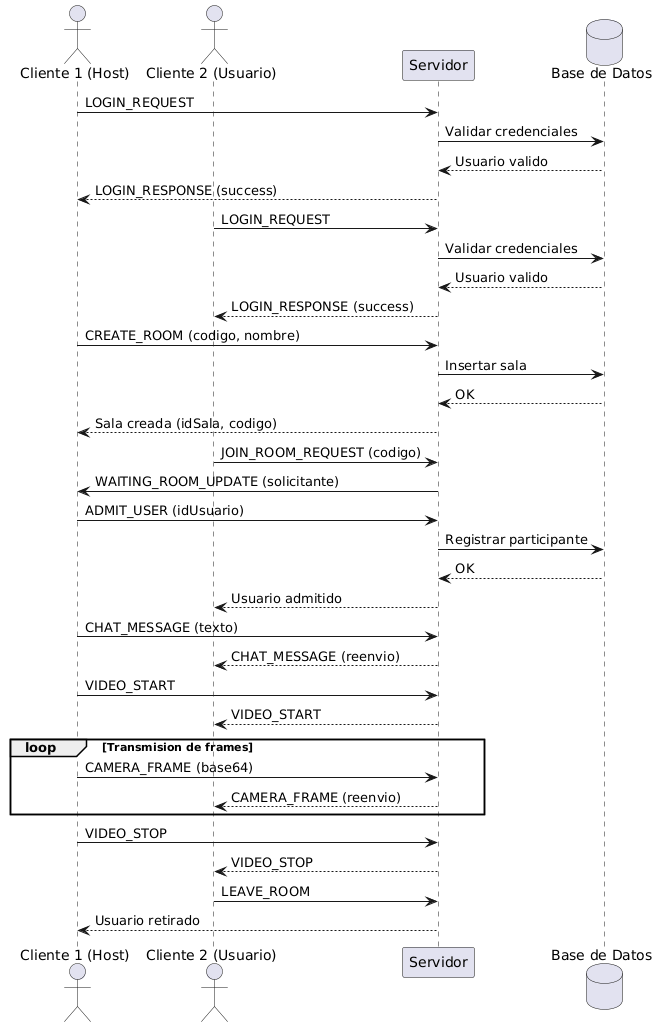
\includegraphics[width=0.9\textwidth]{imagenes/secuencia.png}
    \caption{Diagrama de secuencia del flujo de la aplicaci\'on}
\end{figure}
}{}

\section{Descripci\'on de Clases}

\subsection{Lado del Servidor}

\subsubsection{Protocolo}
\texttt{Servidor/protocolo.py}

Clase de constantes que define todos los tipos de mensaje del protocolo:

\begin{lstlisting}
class Protocolo:
    LOGIN_REQUEST = "LOGIN_REQUEST"
    LOGIN_RESPONSE = "LOGIN_RESPONSE"
    CREATE_ROOM = "CREATE_ROOM"
    JOIN_ROOM_REQUEST = "JOIN_ROOM_REQUEST"
    CHAT_MESSAGE = "CHAT_MESSAGE"
    CAMERA_FRAME = "CAMERA_FRAME"
    FILE_START = "FILE_START"
    FILE_CHUNK = "FILE_CHUNK"
    FILE_END = "FILE_END"
    LEAVE_ROOM = "LEAVE_ROOM"
\end{lstlisting}

\subsubsection{BaseDatos}
\texttt{Servidor/base\_datos.py}

Singleton que gestiona la conexi\'on a SQLite. Inicializa el esquema y los datos de prueba.

\begin{lstlisting}
class BaseDatos:
    _instancia = None

    def __new__(cls, *args, **kwargs):
        if cls._instancia is None:
            cls._instancia = super().__new__(cls)
        return cls._instancia

    def inicializar(self):
        with open("crear_tablas.sql") as f:
            self.conectar().cursor().executescript(f.read())
\end{lstlisting}

\subsubsection{AuthService}
\texttt{Servidor/auth\_service.py}

Valida credenciales consultando la BD con hash SHA-256:

\begin{lstlisting}
class AuthService:
    def validar_login(self, correo, clave):
        password_hash = BaseDatos.hash_clave(clave)
        cursor.execute(
            "SELECT IdUsuario, Nombres, Rol FROM Usuarios "
            "WHERE Correo = ? AND PasswordHash = ? AND Activo = 1",
            (correo, password_hash)
        )
        resultado = cursor.fetchone()
        if resultado:
            return {"status": "success", "idUsuario": ...}
        return {"status": "error", "message": "Credenciales incorrectas"}
\end{lstlisting}

\subsubsection{ManejadorCliente}
\texttt{Servidor/manejador\_cliente.py}

Maneja la comunicaci\'on con un cliente en un hilo separado. El bucle principal lee mensajes JSON delimitados por \verb|\n| y los despacha seg\'un su tipo:

\begin{lstlisting}
class ManejadorCliente:
    def iniciar(self):
        buffer = ""
        while self._conectado:
            datos = self._conexion.recv(4096).decode("utf-8")
            buffer += datos
            while "\n" in buffer:
                linea, buffer = buffer.split("\n", 1)
                mensaje = json.loads(linea)
                self._procesar_mensaje(mensaje)

    def _procesar_mensaje(self, mensaje):
        tipo = mensaje.get("type")
        if tipo == Protocolo.LOGIN_REQUEST:
            self._manejar_login(mensaje)
        elif tipo == Protocolo.CREATE_ROOM:
            self._manejar_crear_sala(mensaje)
        elif tipo == Protocolo.CHAT_MESSAGE:
            self._servidor.reenviar_a_sala(
                mensaje.get("roomCode"), mensaje, self)
\end{lstlisting}

\subsubsection{Servidor}
\texttt{Servidor/servidor.py}

Servidor TCP principal. Acepta conexiones y crea un hilo por cada cliente:

\begin{lstlisting}
class Servidor:
    def iniciar(self):
        BaseDatos().inicializar()
        self._socket = socket.socket(socket.AF_INET, socket.SOCK_STREAM)
        self._socket.bind((self._host, self._puerto))
        self._socket.listen()
        while self._activo:
            conexion, direccion = self._socket.accept()
            manejador = ManejadorCliente(self, conexion, direccion)
            hilo = threading.Thread(target=manejador.iniciar, daemon=True)
            hilo.start()
\end{lstlisting}

\subsection{Lado del Cliente}

\subsubsection{MainApp}
\texttt{Cliente/main.py}

Ventana principal Tkinter. Gestiona la navegaci\'on entre pantallas:

\begin{lstlisting}
class MainApp(tk.Tk):
    def _on_login_exitoso(self, usuario, cliente_socket):
        self._usuario = usuario
        self._cliente_socket = cliente_socket
        self._mostrar_principal()

    def _mostrar_sala(self, codigo_sala, es_host, id_sala):
        self.geometry("900x600")
        self._frame_actual = PantallaSala(
            self, self._usuario, self._cliente_socket,
            codigo_sala, es_host, id_sala, self._salir_sala
        )
        self._frame_actual.pack(fill=tk.BOTH, expand=True)
\end{lstlisting}

\subsubsection{ClienteSocket}
\texttt{Cliente/cliente\_socket.py}

Abstracci\'on del socket TCP con callbacks para despachar mensajes entrantes:

\begin{lstlisting}
class ClienteSocket:
    def _escuchar(self):
        buffer = ""
        while self._conectado:
            datos = self._socket.recv(4096).decode("utf-8")
            buffer += datos
            while "\n" in buffer:
                linea, buffer = buffer.split("\n", 1)
                mensaje = json.loads(linea)
                tipo = mensaje.get("type")
                cb = self._callbacks.get(tipo)
                if cb:
                    cb(mensaje)

    def enviar(self, datos):
        self._socket.send(
            (json.dumps(datos) + "\n").encode("utf-8"))
\end{lstlisting}

\subsubsection{Usuario}
\texttt{Cliente/modelos/usuario.py}

Modelo del usuario autenticado:

\begin{lstlisting}
class Usuario:
    def __init__(self, id_usuario, nombres, correo, rol):
        self._id_usuario = id_usuario
        self._nombres = nombres
        self._correo = correo
        self._rol = rol

    def es_host(self):
        return self._rol.lower() == "host"
\end{lstlisting}

\subsubsection{Mensaje}
\texttt{Cliente/modelos/mensaje.py}

Modelo de mensaje de chat con serializaci\'on a diccionario:

\begin{lstlisting}
class Mensaje:
    def a_dict(self):
        return {
            "type": "CHAT_MESSAGE",
            "roomCode": self._sala_codigo,
            "userId": self._id_usuario,
            "userName": self._nombre_usuario,
            "message": self._contenido
        }
\end{lstlisting}

\subsubsection{LoginFrame}
\texttt{Cliente/pantallas/login.py}

Pantalla de inicio de sesi\'on. Env\'ia \texttt{LOGIN\_REQUEST} al servidor:

\begin{lstlisting}
class LoginFrame(tk.Frame):
    def _procesar_login(self):
        respuesta = self._cliente_socket.enviar_y_recibir({
            "type": "LOGIN_REQUEST",
            "correo": self._entrada_correo.get(),
            "clave": self._entrada_clave.get()
        })
        if respuesta.get("status") == "success":
            usuario = Usuario(respuesta["idUsuario"],
                              respuesta["nombres"], correo,
                              respuesta["rol"])
            self._on_login_exitoso(usuario, self._cliente_socket)
\end{lstlisting}

\subsubsection{PantallaPrincipal}
\texttt{Cliente/pantallas/pantalla\_principal.py}

Men\'u principal con opciones de crear o unirse a una sala:

\begin{lstlisting}
class PantallaPrincipal(tk.Frame):
    def _crear_sala(self):
        codigo = ''.join(random.choices(
            string.ascii_uppercase + string.digits, k=6))
        respuesta = self._cliente_socket.enviar_y_recibir({
            "type": "CREATE_ROOM",
            "nombre": f"Sala de {self._usuario.nombres}",
            "codigo": codigo,
            "idHost": self._usuario.id_usuario
        })
        if respuesta.get("status") == "success":
            self._on_entrar_sala(codigo, True, respuesta["idSala"])
\end{lstlisting}

\subsubsection{PantallaSala}
\texttt{Cliente/pantallas/pantalla\_sala.py}

Pantalla principal de la sala. Integra chat, video y transferencia de archivos:

\begin{lstlisting}
class PantallaSala(tk.Frame):
    def _enviar_mensaje(self):
        texto = self._entrada_msg.get().strip()
        self._cliente_socket.enviar({
            "type": "CHAT_MESSAGE",
            "roomCode": self._codigo_sala,
            "userName": self._usuario.nombres,
            "message": texto
        })

    def _enviar_archivo_thread(self, ruta, nombre, tamano):
        with open(ruta, "rb") as f:
            datos = base64.b64encode(f.read()).decode()
        self._cliente_socket.enviar({
            "type": "FILE_START", "roomCode": self._codigo_sala,
            "fileName": nombre, "fileSize": tamano
        })
        for i in range(0, len(datos), 1500):
            self._cliente_socket.enviar({
                "type": "FILE_CHUNK", "roomCode": self._codigo_sala,
                "fileName": nombre, "data": datos[i:i+1500]
            })
\end{lstlisting}

\subsubsection{PanelVideo}
\texttt{Cliente/pantallas/pantalla\_video.py}

Panel que muestra frames de video desde base64:

\begin{lstlisting}
class PanelVideo(tk.Frame):
    def actualizar_frame(self, datos_b64):
        img_data = base64.b64decode(datos_b64)
        img = Image.open(io.BytesIO(img_data))
        img = img.resize((self._width, self._height), Image.LANCZOS)
        self._imagen_tk = ImageTk.PhotoImage(img)
        self._label_video.config(image=self._imagen_tk, text="")
\end{lstlisting}

\section{Protocolo de Comunicaci\'on}

Los mensajes se env\'ian en JSON sobre TCP, delimitados por \verb|\n|.

\begin{table}[htbp]
    \centering
    \small
    \begin{tabular}{>{\raggedright\arraybackslash}p{4.5cm}p{2.5cm}p{8.5cm}}
    \toprule
    \textbf{Tipo} & \textbf{Direcci\'on} & \textbf{Campos} \\
    \midrule
    LOGIN\_REQUEST   & Cliente $\rightarrow$ Servidor & correo, clave \\
    LOGIN\_RESPONSE  & Servidor $\rightarrow$ Cliente & status, idUsuario, nombres, rol \\
    CREATE\_ROOM     & Cliente $\rightarrow$ Servidor & codigo, nombre, idHost \\
    JOIN\_ROOM\_REQUEST & Cliente $\rightarrow$ Servidor & codigo, idUsuario \\
    WAITING\_ROOM\_UPDATE & Servidor $\rightarrow$ Host & idSala, solicitanteId, solicitanteNombre \\
    ADMIT\_USER      & Host $\rightarrow$ Servidor & idSala, idUsuario \\
    REJECT\_USER     & Host $\rightarrow$ Servidor & idSala, idUsuario \\
    CHAT\_MESSAGE    & Cliente $\rightarrow$ Sala & roomCode, userName, message \\
    FILE\_START      & Cliente $\rightarrow$ Sala & roomCode, fileName, fileSize \\
    FILE\_CHUNK      & Cliente $\rightarrow$ Sala & roomCode, fileName, data \\
    FILE\_END        & Cliente $\rightarrow$ Sala & roomCode, fileName \\
    CAMERA\_FRAME    & Cliente $\rightarrow$ Sala & roomCode, userName, data (base64) \\
    VIDEO\_START     & Cliente $\rightarrow$ Sala & roomCode, userName \\
    VIDEO\_STOP      & Cliente $\rightarrow$ Sala & roomCode, userName \\
    LEAVE\_ROOM      & Cliente $\rightarrow$ Servidor & roomCode \\
    \bottomrule
    \end{tabular}
    \caption{Tipos de mensaje del protocolo}
\end{table}

\section{Manual de Instalaci\'on y Ejecuci\'on}

\subsection{Requisitos}
\begin{itemize}
    \item Python 3.10 o superior
    \item Pillow (instalar con \texttt{pip install -r requirements.txt})
    \item Opcional: OpenCV (\texttt{pip install opencv-python}) o ffmpeg
\end{itemize}

\subsection{Ejecuci\'on}
\begin{enumerate}
    \item Iniciar el servidor:
    \begin{lstlisting}
python -m Servidor.servidor
    \end{lstlisting}
    \item Iniciar uno o m\'as clientes:
    \begin{lstlisting}
python -m Cliente.main
    \end{lstlisting}
\end{enumerate}

\subsection{Datos de Prueba}

\begin{table}[htbp]
    \centering
    \begin{tabular}{p{2.5cm}p{3cm}p{1.5cm}p{1.5cm}}
    \toprule
    \textbf{Nombre} & \textbf{Correo} & \textbf{Clave} & \textbf{Rol} \\
    \midrule
    Luis Tasayco  & luis@email.com   & 123456 & Host \\
    Ana Torres    & ana@email.com    & 123456 & Usuario \\
    Carlos Ruiz   & carlos@email.com & 123456 & Usuario \\
    \bottomrule
    \end{tabular}
    \caption{Usuarios de prueba}
\end{table}

\section{Conclusiones}

\begin{itemize}
    \item Se implement\'o un prototipo funcional de videoconferencia con arquitectura cliente-servidor.
    \item Los sockets TCP con protocolo JSON proporcionan una base s\'olida para comunicaci\'on en tiempo real.
    \item La POO permiti\'o organizar el c\'odigo en clases especializadas con responsabilidades claras.
    \item El patr\'on Singleton garantiza una \'unica instancia de conexi\'on a la base de datos.
    \item La concurrencia con hilos permite atender m\'ultiples clientes simult\'aneamente.
    \item La transmisi\'on de video se logr\'o mediante captura, compresi\'on JPEG y codificaci\'on base64.
\end{itemize}

\end{document}
